\chapter{Psalm 11}

\begin{figure}
  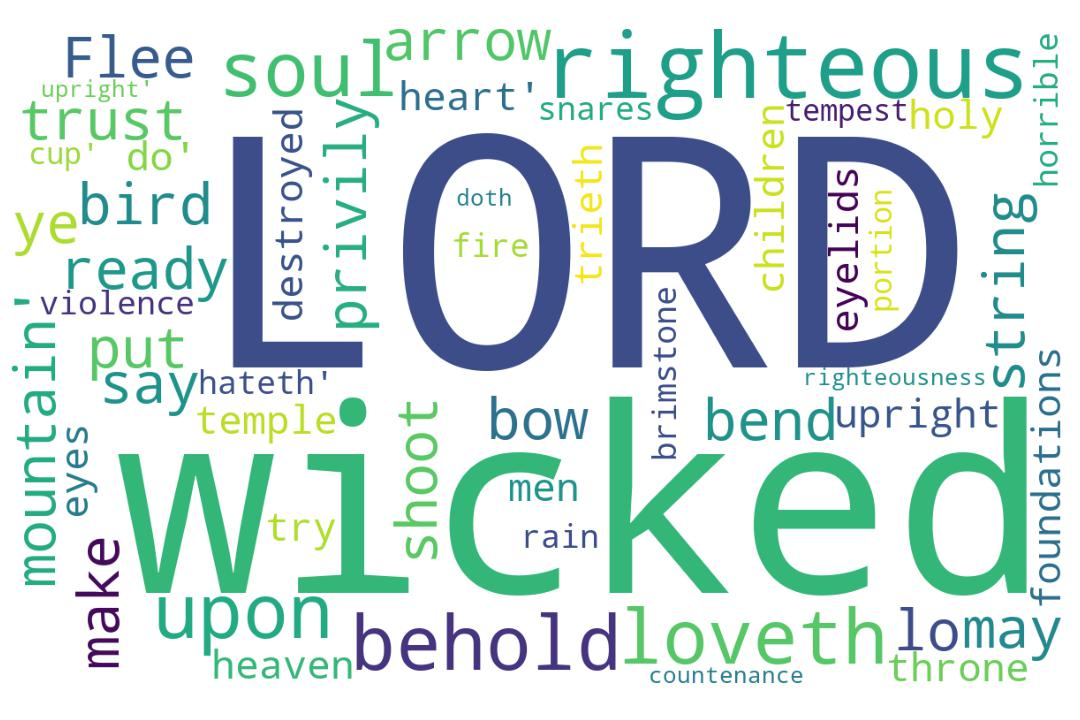
\includegraphics[width=\linewidth]{19OT-Psalms/Psalm11-WordCloud.jpg}
  \caption{Psalm 11 Word Cloud}
  \label{fig:Psalm 11 word Cloud}
\end{figure}

\marginpar{\scriptsize \centering \fcolorbox{bone}{lime}{\textbf{GOD IS WATCHING}}\\ (Psalm 11:1-7)     \begin{compactenum}[I.]
    \item He is \textbf{Interested in Paths of Mankind} \index[scripture]{Psalms!Psa 011:01}(Psa 11:1)
    \item He \textbf{Investigates the Manner of People} \index[scripture]{Psalms!Psa 011:01}(Psa 11:1)
    \item He \textbf{Intervenes is the Plans of Man} \index[scripture]{Psalms!Psa 011:02}(Psa 11:2)
    \item He \textbf{Interferes in the Programs of Evil} \index[scripture]{Psalms!Psa 011:02}(Psa 11:2)
    \item He is \textbf{Involved in the Progression of History} \index[scripture]{Psalms!Psa 011:04}(Psa 11:4)
    \item He \textbf{Invests in His Priorities}  \index[scripture]{Psalms!Psa 001:04}(Psa 11:4)
    \item He \textbf{Inhabits His Property} \index[scripture]{Psalms!Psa 011:06}(Psa 11:6)
\end{compactenum}}

\marginpar{\scriptsize \centering \fcolorbox{bone}{yellow}{\textbf{A TRIP TO SELAH PETRA}}\\ (Psalm 11:1-7)     
\begin{compactenum}[I.]
    \item The \textbf{Flight} \index[scripture]{Psalms!Psa 011:01}(Psa 11:1)
    \item The \textbf{Foe} \index[scripture]{Psalms!Psa 011:02}(Psa 11:2)
    \item The \textbf{Foundations} \index[scripture]{Psalms!Psa 011:03}(Psa 11:3)
    \item The \textbf{Fitness} Test \index[scripture]{Psalms!Psa 011:05}(Psa 11:5)
    \item The \textbf{Furor} Test \index[scripture]{Psalms!Psa 011:05}(Psa 11:5)
    \item The \textbf{Fire} \index[scripture]{Psalms!Psa 011:06}(Psa 11:6)
    \item The \textbf{Faithfulness} (of the Lord) \index[scripture]{Psalms!Psa 011:07}(Psa 11:7)
\end{compactenum}}



\footnote{\textcolor[cmyk]{0.99998,1,0,0}{\hyperlink{TOC}{Return to end of Table of Contents.}}}\footnote{\href{https://audiobible.com/bible}{\textcolor[cmyk]{0.99998,1,0,0}{Psalms Audio}}}\textcolor[cmyk]{0.99998,1,0,0}{To the chief Musician, \emph{A Psalm} of David.}\\
\\
\textcolor[cmyk]{0.99998,1,0,0}{In the LORD put I my trust: how say ye to my soul, \fcolorbox{bone}{lime}{Flee} \emph{as} a bird to your mountain?}\footnote{\textbf{Matthew 24:15-22} - \textcolor{red}{When ye therefore shall see the abomination of desolation, spoken of by Daniel the prophet, stand in the holy place, (whoso readeth, let him understand:)} [16] \textcolor{red}{Then let them which be in Judaea flee into the mountains:} [17] \textcolor{red}{Let him which is on the housetop not come down to take any thing out of his house:} [18] \textcolor{red}{Neither let him which is in the field return back to take his clothes.} [19] \textcolor{red}{And woe unto them that are with child, and to them that give suck in those days!} [20] \textcolor{red}{But pray ye that your flight be not in the winter, neither on the sabbath day:} [21] \textcolor{red}{For then shall be great tribulation, such as was not since the beginning of the world to this time, no, nor ever shall be.} [22] \textcolor{red}{And except those days should be shortened, there should no flesh be saved: but for the elect’s sake those days shall be shortened.}}\footnote{\textbf{Mark 13:14-20} - \textcolor{red}{But when ye shall see the abomination of desolation, spoken of by Daniel the prophet, standing where it ought not, (let him that readeth understand,) then let them that be in Judæa flee to the mountains:} [15] \textcolor{red}{And let him that is on the housetop not go down into the house, neither enter therein, to take any thing out of his house:} [16] \textcolor{red}{And let him that is in the field not turn back again for to take up his garment.} [17] \textcolor{red}{But woe to them that are with child, and to them that give suck in those days!} [18] \textcolor{red}{And pray ye that your flight be not in the winter.} [19] \textcolor{red}{For in those days shall be affliction, such as was not from the beginning of the creation which God created unto this time, neither shall be.} [20] \textcolor{red}{And except that the Lord had shortened those days, no flesh should be saved: but for the elect’s sake, whom he hath chosen, he hath shortened the days.}}
[2] \textcolor[cmyk]{0.99998,1,0,0}{For, lo, the wicked bend \emph{their} bow, they make ready their arrow upon the string, that they may privily shoot at the upright in heart.}
[3] \textcolor[cmyk]{0.99998,1,0,0}{If the foundations be destroyed, what can the righteous do?}
[4] \textcolor[cmyk]{0.99998,1,0,0}{The LORD \emph{is} \fcolorbox{bone}{lime}{in his holy temple}, the LORD'S throne \emph{is} in heaven: his eyes behold, \fcolorbox{bone}{lime}{his eyelids try}, the children of men.}
[5] \textcolor[cmyk]{0.99998,1,0,0}{The LORD trieth the righteous: but the wicked and him that loveth violence his soul hateth.}
[6] \textcolor[cmyk]{0.99998,1,0,0}{Upon the wicked he shall rain snares, fire and brimstone, and an horrible tempest: \emph{this} \emph{shall} \emph{be} the portion of their cup.}
[7] \textcolor[cmyk]{0.99998,1,0,0}{For the righteous LORD loveth righteousness; his countenance doth behold the upright.}

